\documentclass[a4paper,11pt, french]{article}
\usepackage[top=2.5cm, bottom=2.5cm, left=2.5cm, right=2.5cm]{geometry} % marges

% French
\usepackage[utf8x]{inputenc}
\usepackage[T1]{fontenc}
\usepackage[french]{babel}


% Packages à importer

\usepackage{lmodern, graphicx, tikz, pgfplots}
\usepackage{graphicx,amssymb,amstext,amsmath}
\usepackage{fancyhdr, url, ifthen, multirow}
\usepackage{subfig, float, caption}
\usepackage{array}
\usepackage{color, colortbl}
\usepackage{hyperref}

\pgfplotsset{compat=1.11}

%Color defining
\definecolor{Gray}{gray}{0.9}

\begin{document}
%-----------------------------------------------------------
% page de couverture

\newcommand{\HRule}{\rule{\linewidth}{0.5mm}}

\fancyhf{} %clear all headers and footers fields
\fancyhead[R]{\thepage} %prints the page number on the right side of the header
\fancyhead[L]{Rapport de laboratoire CSTR}


\pagestyle{fancy}
\thispagestyle{empty}
\begin{titlepage}
\begin{center}


\includegraphics[width=0.15\textwidth]{pictures/logo.JPG}~\\[1cm]

\textsc{\LARGE Université Catholique de Louvain}\\[1.5cm]

\textsc{\Large Projet 3}\\[0.5cm]

% Title
\HRule \\[0.4cm]
{ \huge \bfseries Rapport de laboratoire CSTR\\[0.4cm] }

\HRule \\[1.5cm]

% Author and supervisor
\begin{minipage}{0.4\textwidth}
\begin{flushleft} \large
\textbf{Groupe \textsc{11.64}} \\
\textsc{Asselberghs} Paul \\
\textsc{Bertin} Brice \\
\textsc{Couplet} Adrien \\
\textsc{Crepeulandt} Grégory \\
\textsc{Gatin} Anthony \\
\textsc{Gennart} Antoine \\
\textsc{Gillard} Juline \\
\textsc{Martin} Pierre


\end{flushleft}
\end{minipage}
\begin{minipage}{0.4\textwidth}
\begin{flushright} \large
%\emph{Tuteur:} \\
%David \textsc{Cordova}
\end{flushright}
\end{minipage}

\setcounter{tocdepth}{2}
\tableofcontents % table des matières, totalement automatique ;)

\vfill

% Bottom of the page
{\large \today}
\end{center}
\end{titlepage}
%-----------------------------------------------------------
% début du document numéroté
\clearpage
\pagenumbering{arabic}
\newpage
%-----------------------------------------------------------

\thispagestyle{empty}


%\newpage

% Début du document, à séparer en plusieurs parties pré-définies
\section{Objectif}
\begin{itemize}
	\item Compréhension de la notion de procédé en continu;
	\item Description de la phase transitoire au démarrage du procédé;
	\item Mesure de débits;
	\item Bilan de masse sur l'unité de dilution;
	\item Présentation graphique et discussion de résultats dans un rapport structuré.
\end{itemize}

\section{Matériel et méthode}
	\subsection{Matériel}
		\begin{itemize}
			\item Bouteille de grenadine (1L) x3
			\item Bouteille de sirop de Menthe (1L) x3
			\item Tubes à transvaser x6
			\item Réservoirs (21cm x 20xcm x 18 cm) x4
			\item Petit réacteur CSTR (Berlin gradué avec évacuation à 920 ml dans notre cas) x2
			\item Mélangeur magnétique x2
			\item Chronomètre x2
			\item Pipettes $\pm$40
			\item Réfractomètre
			\item Tube gradué x2	
		\end{itemize}
		\begin{figure}[h]
			\centering
			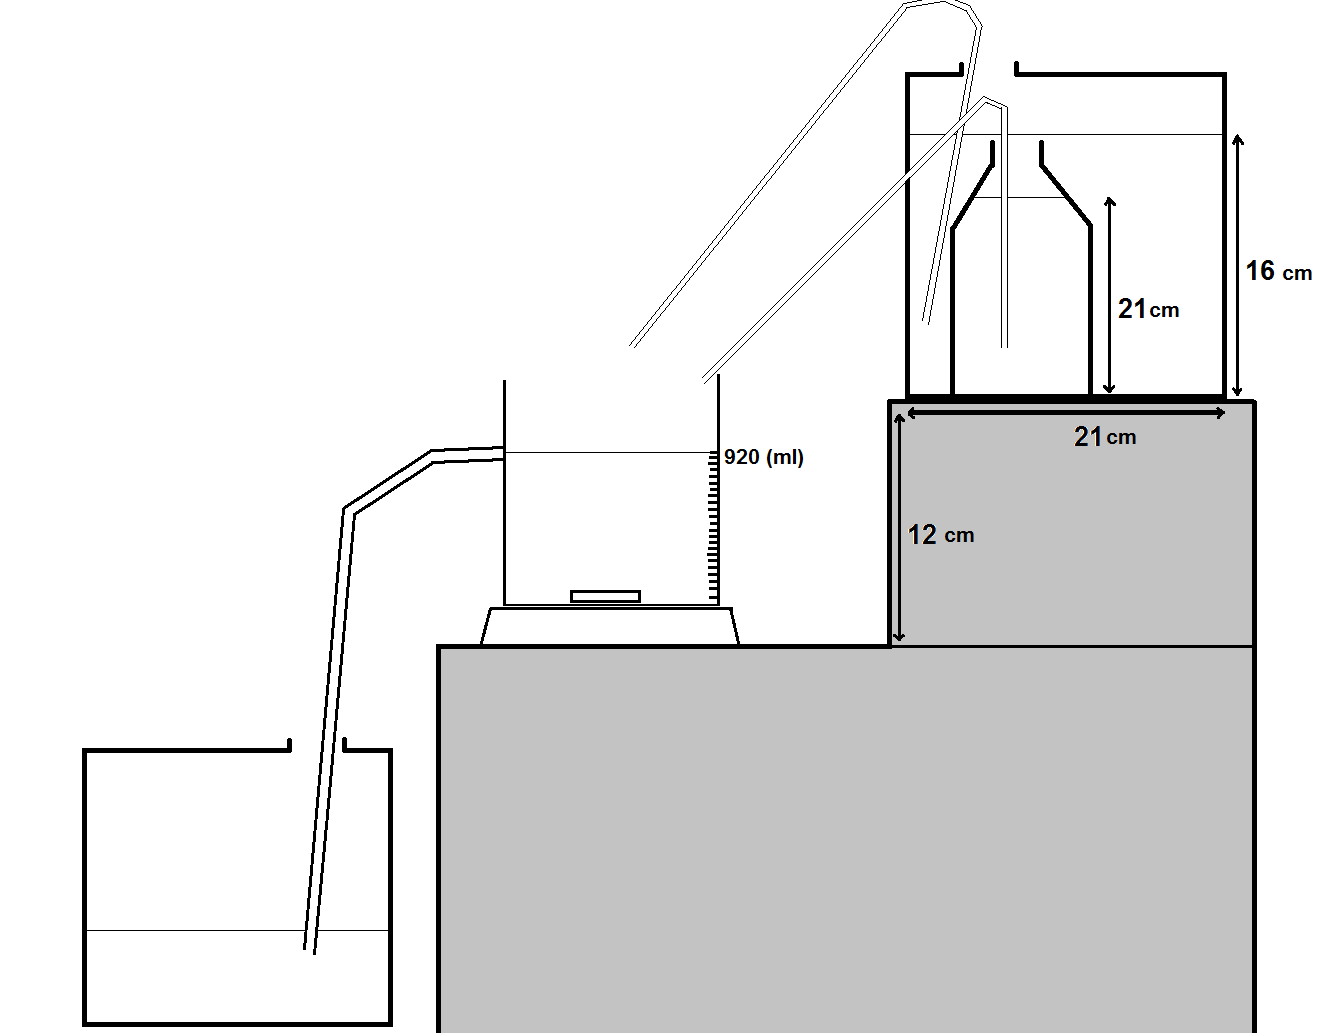
\includegraphics[width=0.7\textwidth]{pictures/materiel.png}
			\caption{Disposition du matériel utilisé}
		\end{figure}	
		
	\subsection{Mode de régulation des débits}
		\subsubsection{Méthode utilisée}
			\begin{enumerate}
				\item Lancement de l'écoulement par appel d'air dans le tube.
				\item Le liquide s'écoule dans un tube gradué. L'opération est chronométrée.
				\item Tous les 10 ml le temps est noté. 
				\item Le débit correspond à $\frac{V}{t}$
				\item Pour le résultat final, nous prenons la valeur moyenne des débits mesurés.
			\end{enumerate}
			\textbf{Remarque :} Afin de garder les débits constants, nous avons veillé à ce que le système reste immobile.
			
	\subsection{Mesure par réfractométrie}
		\subsubsection{Principe de fonctionnement}
			La réfractométrie est une technique de mesure de l'indice de réfraction d'un matériau. Le réfractomètre utilisé pour nos mesures est de type portable et mesure en degrés Brix ($^{\circ}$B) la fraction de saccharose en g pour 100g de liquide. La mesure se fait à l'aide d'un prisme à indice de réfraction élevé. Sur base du phénomène de réfraction, la lumière, au passage de l'échantillon au prisme, est déviée de sa trajectoire. (Voir figure \ref{refractometrie})
			\begin{itemize}
				\item La réfraction est grande lorsque la teneur en sucre de l'échantillon est faible.
				\item Inversement, la réfraction est faible lorsque la teneur en sucre est élevée.
			\end{itemize}
			\textbf{Remarque :} Le réfractomètre utilisé dispose d'une correction automatique de la températue
			\begin{figure}[h]
				\centering
				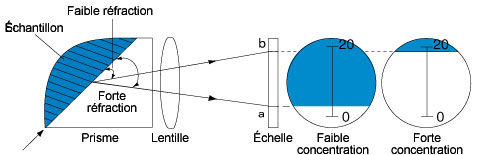
\includegraphics[width=1.0\textwidth]{pictures/refractometre.jpg}
				\caption{Fonctionnement d'un réfracomètre\label{refractometrie}\protect\footnotemark}
			\end{figure}
			\footnotetext{Source : \url{http://www.mesurez.com/refractometre-principe-mode-emploi.html}}
		\subsubsection{Méthode utilisée}
			\begin{enumerate}
				\item Prélevement régulier du mélange dans le réacteur (systématiquement au même endroit, au fond au bord).
				\item Mesure au réfractomètre de la concentration en saccharose de l'échantillon.
			\end{enumerate}
			\textbf{Remarque :} Pour mesurer le taux de sucre de la grenadine/menthe (trop élevé pour le réfractomètre), nous l'avons diluée dans de l'eau.
	\subsection{Bilan de masse}
		\subsubsection{Méthode utilisée}
			Pour les bilans de volumes totaux, nous avons regardé les débits des différents liquides que nous avions. Nous avons ensuite comparé les volumes finaux obtenus dans les bidons et dans le réacteur.
			
			Pour les bilans de masse, nous avons regardé la quantité de sucre dans les solutés à partir de l'étiquette. A partir des débits, nous avons pu déterminer quelle quantité de sucre entrait dans le réacteur. Ensuite, grâce à la mesure de réfractométrie nous avons pu comparer les résultats obtenus.  

\section{Résultats}
	\subsection{Calcul du débit}
	\begin{table}[h!]
		\centering
		\begin{footnotesize}
		\subfloat{
			\centering
			\begin{tabular}{|c|c|c|}\hline
				\rowcolor{Gray}	
				\multicolumn{3}{|c|}{\textbf{Débit menthe (soluté)}} \\ \hline
				Temps & Volume & Débit \\ 
				$[s]$ & $[ml]$ & $[ml/s]$ \\ \hline
				52 & 20 & 0.38 \\
				98 & 30 & 0.31 \\
				105 & 40 & 0.38 \\ \hline
				\multicolumn{2}{|c|}{\textbf{Moyenne}} & 0.35 \\ \hline
			\end{tabular}
		}
		\subfloat{
			\centering
			\begin{tabular}{|c|c|c|}\hline
				\rowcolor{Gray}	
				\multicolumn{3}{|c|}{\textbf{Débit grenadine (soluté)}} \\ \hline
				Temps & Volume & Débit \\ 
				$[s]$ & $[ml]$ & $[ml/s]$ \\ \hline
				59 & 20 & 0.34 \\
				93 & 30 & 0.32 \\
				126 & 40 & 0.32 \\ \hline
				\multicolumn{2}{|c|}{\textbf{Moyenne}} & 0.33 \\ \hline
			\end{tabular}
		}
		\subfloat{
			\centering
			\begin{tabular}{|c|c|c|}\hline
				\rowcolor{Gray}	
				\multicolumn{3}{|c|}{\textbf{Débit eau (solvant)}} \\ \hline
				Temps & Volume & Débit \\ 
				$[s]$ & $[ml]$ & $[ml/s]$ \\ \hline
				9 & 30 & 3 \\
				12 & 40 & 3.3 \\
				15 & 50 & 3.3 \\
				18 & 60 & 3.3 \\ \hline
				\multicolumn{2}{|c|}{\textbf{Moyenne}} & 3.3 \\ \hline
			\end{tabular}
		}
		\end{footnotesize}
		\caption{Tableaux des mesures de débits \label{mesures}}
	\end{table}		
\subsection{Graphique}
\begin{figure}[h!]
	\begin{minipage}[m]{.3\textwidth}
		\centering\begin{scriptsize}
		\begin{tabular}{|c|c|}\hline\rowcolor{Gray}
			Temps & Taux \\ \rowcolor{Gray}
			$[min]$ & $[^\circ B]$ \\ \hline
			0 & 0.2 \\
			1 & 1.4 \\
			2 & 2.3 \\
			3 & 3.1 \\
			4 & 3.8 \\
			5 & 4.1 \\
			6 & 4.6 \\
			8 & 5.0 \\
			10 & 5.3 \\
			12 & 5.7 \\
			15 & 5.4 \\
			20 & 5.8 \\
			25 & 5.9 \\
			30 & 5.9 \\
			35 & 5.9 \\
			40 & 6.2 \\
			45 & 5.9 \\ \hline
		\end{tabular}\end{scriptsize}
	\end{minipage}
	\begin{minipage}[m]{.5\textwidth}
		\centering
		\begin{tikzpicture}
			\begin{axis}[
				height=6cm,
				width=10cm,
				grid=major,
				legend pos=south east,
				xlabel={Temps $[min]$},
				ylabel={Taux de saccharose $[^\circ B]$},
			]
			\addplot coordinates {
				(0, 0.2)
				(1, 1.4)
				(2, 2.3)
				(3, 3.1)
				(4, 3.8)
				(5, 4.1)
				(6, 4.6)
				(8, 5.0)
				(10, 5.3)
				(12, 5.7)
				(15, 5.4)
				(20, 5.8)
				(25, 5.9)
				(30, 5.9)
				(35, 5.9)
				(40, 6.2)
				(45, 5.9)
			};
			\addlegendentry{Taux de saccharose}
			\end{axis}
		\end{tikzpicture}
	\end{minipage}
	\caption{Taux de saccharose par rapport au temps (Grenadine) \label{grenad}}
\end{figure}
\begin{figure}[h!]
	\begin{minipage}[m]{.3\textwidth}
		\centering\begin{scriptsize}
		\begin{tabular}{|c|c|}\hline \rowcolor{Gray}
			Temps & Taux \\ \rowcolor{Gray}
			$[min]$ & $[^\circ B]$ \\ \hline
			0 & 0.0 \\
			1 & 2.0 \\
			2 & 3.0 \\
			3 & 4.8 \\
			4 & 5.0 \\
			5 & 5.8 \\
			6 & 6.2 \\
			8 & 7.0 \\
			10 & 7.4 \\
			12 & 8.0 \\
			15 & 8.3 \\
			20 & 8.8 \\
			25 & 8.9 \\
			30 & 9.0 \\
			35 & 9.0 \\
			40 & 9.0 \\
			45 & 9.0 \\ \hline
		\end{tabular}\end{scriptsize}
	\end{minipage}
	\begin{minipage}[m]{.5\textwidth}
		\centering
		\begin{tikzpicture}
			\begin{axis}[
				height=6cm,
				width=10cm,
				grid=major,
				legend pos=south east,
				xlabel={Temps $[min]$},
				ylabel={Taux de saccharose $[^\circ B]$},
			]

			\addplot coordinates {
				(0, 0.0)
				(1, 2.0)
				(2, 3.0)
				(3, 4.8)
				(4, 5.0)
				(5, 5.8)
				(6, 6.2)
				(8, 7.0)
				(10, 7.4)
				(12, 8.0)
				(15, 8.3)
				(20, 8.8)
				(25, 8.9)
				(30, 9.0)
				(35, 9.0)
				(40, 9.0)
				(45, 9.0)
			};
			\addlegendentry{Taux de saccharose}
			\end{axis}
		\end{tikzpicture}
	\end{minipage}
	\caption{Taux de saccharose par rapport au temps (Menthe) \label{menth}}
\end{figure}

\subsection{Bilan de masse en régime stationnaire}
	\paragraph*{Vérification des volumes obtenus}
		\begin{align*} 
			V_\text{total} &= V_\text{initial} + V_\text{sortie} \\
						   &= 0.920 + ( 2.1 \cdot 2.1 \cdot 1.75 ) \\
						   &= 0.920 + 7.715 \\
						   &= 8.6375\ L \\
			V_\text{débit} &= (0.33 + 3.3) \cdot 45 \cdot 60 = 10.721\ L 
		\end{align*}
		On remarque que les résultats obtenus sont fort différents mais appartiennent au même ordre de grandeur.
	\paragraph*{Bilan de masse (mélange grenadine)}\mbox{} \\
		\begin{table}[h]
			\centering
			\begin{tabular}{|l|l|}\hline
				Résultats mesurés par réfractométrie & 5.9g de sucre pour 100ml d'eau\\\hline
				Selon les ingrédients & 68.8g de sucre pour 100ml de grenadine.\\\hline
				Selon les débits & 5.7g de sucre pour 100ml de mélange\\\hline
			\end{tabular}
		\end{table}
		$$D_v = 0.33\ ml/s \Rightarrow D_{m,\text{sucre}} = 0.227\ g/s \qquad V_\text{total} = 10.721\ L$$
		$$m_\text{sucre} = D_{m,\text{sucre}} \cdot 45 \cdot 60 = 613\ g$$
	\paragraph*{Bilan de masse (mélange menthe)}\mbox{} \\
		\begin{table}[h]
			\centering
			\begin{tabular}{|l|l|}\hline
				Résultats mesurés par réfractométrie & 9.0g de sucre pour 100ml d'eau\\\hline
				Selon les ingrédients & 68.8g de sucre pour 100ml de menthe.\\\hline
				Selon les débits & 6.5g de sucre pour 100ml de mélange\\\hline
			\end{tabular}
		\end{table}
		$$D_v = 0.38\ ml/s \Rightarrow D_{m,\text{sucre}} = 0.261\ g/s \qquad V_\text{total} = 10.856\ L$$
		$$m_\text{sucre} = D_{m,\text{sucre}} \cdot 45 \cdot 60 = 705.8\ g$$
		
		

\section{Discussion}
	\subsection*{a) Comparaison des deux expériences}
On remarque grâce aux graphiques des figures \ref{grenad} et \ref{menth} que la valeur limite du taux de saccharose entre les deux expériences (menthe et grenadine) est différente. Nous expliquons cela par une différence de débit entre la menthe et la grenadine, le débit de menthe étant plus élevé (voir table \ref{mesures}).

	\subsection*{b) Ce qu'on peut en tirer comme loi(s) générale(s) sur la phase transitoire}
On remarque que lors de la phrase transitoire le taux de sucre augmente de manière exponentielle jusqu'à la phase stationnaire. Dans la phase transitoire, contrairement au régime stationnaire, on remarque que le taux de sucre varie avec le temps.

	\subsection*{c) Influence du volume du réacteur (avantages / désavantages)}

Un grand réacteur à l'avantage d'être stable (il fallait moins souvent remettre de l'eau dans le bidon pour garder un débit constant) par contre il a le désavantage de demander un plus grande quantité initiale.

	\subsection*{d) Comparaison d'un procédé en continu par rapport à un procédé en batch}
Un procédé en continu est se déroule dans des conditions identiques tout au long du déroulement (températures, pression, quantité de soluté, quantité de solvant, ...). Il y a toujours le même apport en solvant et soluté à l'entrée du réacteur, et le même produit qui en sort fini.

Un procédé en batch, aussi appelé procédé discontinu est surtout utilisé de manière expérimentale, lors que des petites quantités, précises sont requises. Dans ce genre de procédé, les conditions peuvent changer (température, pression, masses, ...).

\begin{table}[h]\centering
\begin{tabular}{|m{0.48\textwidth}|m{0.48\textwidth}|}\hline
	\rowcolor{Gray}	
	\begin{center}Avantages d'un \textbf{procédé continu}\end{center} & \begin{center}Avantages d'un procédé en \textbf{batch}\end{center} \\\hline
	- Déroulement automatique & - Pas de surveillance constante du procédé \\
	- Phase transitoire observable avec précision & - Quantités précises produite \\
	- Qualité constante & - Pas de contrôle des flux \\
	- Production sans arrêt & - Changement de température possible \\\hline
\end{tabular}
\end{table}

	\subsection*{e) Que se passerait-il si le procédé ce déroulerait lentement ?}
La phase transitoire serait très longue.

	\subsection*{f) Que se passerait-il si la réaction était incomplète ?}
Il y aurait des réactifs et des produits présents simultanéments dans le réacteur. 

\end{document}


